\documentclass[8pt]{beamer}
\geometry{paperwidth=180mm,paperheight=105mm}


\usepackage{amsmath}
\usepackage{wrapfig}
\usepackage{tikz-cd}
\usepackage{url}
\title{Seifert -- Van Kampen Theorem, Applications}
\author{Yahya Tamur}

\begin{document}

  \frame{\titlepage}
  \begin{frame}
    \frametitle{Groups; generators and relations}
    \begin{columns}
      \begin{column}[T]{0.5\textwidth}
        \begin{itemize}
          \item A group is a set of elements $G$, with a $. : GxG \rightarrow G$
            such that:
            \[(a.b).c = a.(b.c)\]
            There's an identity element $1$ such that for all $a$,
            \[1.a = a.1 = a\]
            For all $a$, there's an inverse element $a^{-1}$ such that:
            \[a^{-1}.a = a.a^{-1} = 1\]
          \item Notably, it doesn't have to be commutative ($a.b$ isn't
            necessarily $b.a$).\pause
          \item Common examples include invertible functions under composition,
            integers under addition (but not multiplication), positive rationals
            under multiplication.\pause
          \item Another example is the one-element group $\{1\}$ with $1.1 = 1$.
            \pause
          \item A function between groups that preserves products, identity, and
            inverses -- $\sigma(a.b) = \sigma(a).\sigma(b)$, $\sigma(1) = 1$,
            $\sigma(a^{-1}) = \sigma(a)^{-1}$ is called a homomorphism. These
            have other special properties that can be derived.\pause
          \item A set ${a,b,...}$ generates a group $G$ if every element can be
            written in as a finite combination of elements (or inverses of
            elements) in the group. Ex. ${1}$ generates integers under addition,
            prime numbers generate positive rationals under multiplication.
            \pause

        \end{itemize}
      \end{column}
      \begin{column}[T]{0.5\textwidth}
        \begin{itemize}
          \item Every group has a generator -- the set of all elements in the
            group.\pause
          \item Given a set of elements, you can define the group of finite
            sequences of elements (and inverses of elements) in the set under
            concatenation. For example:
            \[(a,b,c^{-1}). (c,a^{-1}) = (a,b,a^{-1})\]
            \[(a,b,c).(a,b,c)^{-1} = (a,b,c).(c^{-1},b^{-1},a^{-1}) = ()\]
            This is called the free group of the set.\pause
          \item
            Then, if you have any group that's generated by that set, there's a
            surjective homomorphism from the free group onto the group, defined
            as
            \[\sigma((x)) = x\]
            and extended to other elements using properties of homomorphisms:
            \[\sigma((a,b,c,a^{-1})) = \sigma((a)).\sigma((b)).\sigma((c)).
                \sigma((a^{-1})) = a.b.c.a^{-1}\]\pause
          \item By the First Isomorphism Theorem, any group is the free group of
            its generators quotiented by the kernel of this homomorphism.\pause

        \end{itemize}
      \end{column}
    \end{columns}
  \end{frame}

  \begin{frame}
    \frametitle{Groups; generators and relations}
    \begin{columns}
      \begin{column}[T]{0.5\textwidth}
        \begin{itemize}

          \item A presentation of a group by its generators and relations
            is essentially the free group, together with a few equivalences:
            \pause
          \item $\langle a,b:a^5,b^3\rangle $ means the free group $\langle a,b
            \rangle $, but $a^5$ and $b^3$ also have to be equal to the
            identity.\pause
          \item This can be expressed as $\langle a,b\rangle $ divided by the
            smallest normal subgroup that contains $a^5$ and $b^3$.\pause
          \item If $G$ is any group generated by $a$ and $b$, with
            $a^5 = b^3 = 1$, we can try to define a homomorphism
            \[\sigma((a)) = a, \sigma((b)) = b\]
            And, this is well-defined, even though some sequences might be
            equivalent in $\langle a,b:a^5,b^3\rangle $ without being equal,
            because whenever terms cancel out in $\langle a,b:a^5,b^3\rangle $,
            they cancel out in $G$:
            \[(a,a,a,b,b,b,a,a) = (a,a,a,a,a) = 1\]
            \[\sigma((a,a,a,b,b,b,a,a)) = aaabbbaa \in G = aaaaa = 1\]\pause
          \item So, for any group generated by the generators and satisfying the
            relations, there's a surjective homomorphism from the presentation
            onto the group.

        \end{itemize}
      \end{column}
      \begin{column}[T]{0.5\textwidth}
        \begin{itemize}
          \item Since there's a surjective homomorphism from the free group of a
            set of generators to any group, we can express any group as a set of
            generators and relations (choose the whole kernel of the
            homomorphism for example).\pause
          \item Note: Some relations might be simplified by adding an equal
            sign:
            \[\langle a,b:aba^{-1}, b^2\rangle  = \langle a,b:ab = a, b^2\rangle \]
        \end{itemize}
      \end{column}
    \end{columns}
  \end{frame}

  \begin{frame}
    \frametitle{Fundemental Groups}
    \begin{columns}
      \begin{column}[T]{0.5\textwidth}
        \begin{itemize}
          \item<1-> Let $X$ be a topological space, and $x_0$ be any point in it.

          \item<2-> A continuous function $f:[0,1] \rightarrow X$ represents a curve
            in $X$. If $f(0) = f(1) = x_0$, we'll call it a loop.

          \item<4-> Define equivalence classes where $f$ is equivalent to $g$ if
            the loops can be continuously deformed into each other. We'll refer
            to these equivalence classes as paths. If $f$ is a loop, and $a$ is
            the path $f$ is in, I'll denote $a = [f]$.
          \item<5-> In $\mathbb{R}^2$, $x_0 = (0,0)$, any two loops are equivalent,
            and there's only one path.
            In $\mathbb{R}^2 - (0,0)$, $x_0 = (1,0)$, the two loops on the right
            aren't equivalent.
          \item<6-> More rigorously, $f \sim g  $ iff there's a continuous $F: [0,1]x
            [0,1] \rightarrow X$ where $F(0,t) = f(t)$, $F(1,t) = g(t)$, and
            $F(s,0) = F(s,1) = x_0$
          \item<7-> Given two loops $f$ and $g$, we can compose them as follows:
            \[f . g (t) = \begin{cases} f(2t) & 0 \leq t \leq \frac{1}{2} \\
                                        g(2t-1) & \frac{1}{2} \leq t \leq 1 \\
            \end{cases}\]
            Then, $(f.g).h \neq f.(g.h)$, but $(f.g).h \sim f.(g.h)$. Also, if
            $f \sim g$, $f . h \sim g . h$ for any  $h$.
          \item<8-> We can define an identity element as $i(t) = x_0$ and inverse
            element as $f^{-1}(t) = f(1-t)$. (Again, $f.f^{-1} \neq 1$ as loops
            but $[f].[f^{-1}] = [f^{-1}].[f] = 1$).
        \end{itemize}
      \end{column}
      \begin{column}[T]{0.5\textwidth}<3->
        \begin{center}
        \includegraphics[width=0.9\textwidth]{img/fgroup-intro.JPG}
        \end{center}
      \end{column}
    \end{columns}
  \end{frame}
  \begin{frame}
    \frametitle{Fundemental Groups}
    \begin{columns}
      \begin{column}[T]{0.5\textwidth}
        \begin{itemize}
          \item<1-> So, paths in $X$ with base point $x_0$ under this operation is a
            group, called the $\pi(X)$. The base point usually doesn't matter,
            since the groups are usually the same regardless of the base point.
          \item<2-> It can be proven that in $\mathbb{R}^2 - (0,0)$, any two loops
            that go around the center the same number of times are equivalent.
            So, if $a$ is the path that represents going aroung once clockwise,
            the group $\pi(\mathbb{R}^2 - (0,0))$ is $\langle a\rangle $, so
            $a^n$ for any $n \in \mathbb{Z}$.
            \pause
          \item<4-> Here, $a^{-n}$ signifies going around counterclockwise $n$ times
            and $a^0$ signifies not going around the point. Then,
            \[a^w . a^z = a^{w+z}\]
        \end{itemize}
      \end{column}
      \begin{column}[T]{0.5\textwidth}<3->
        \begin{center}
        \includegraphics[width=0.7\textwidth]{img/ex-pi-R2-0.JPG}
        \end{center}
      
      \end{column}
    \end{columns}
  \end{frame}
  \begin{frame}
    \frametitle{Fundemental Groups}
    \begin{columns}
      \begin{column}[T]{0.5\textwidth}
        \begin{itemize}
          \item<1-> Let $\sigma$ be a continuous function between $X$ and $Y$.
          \item<2-> Then, for loops $f,g : [0,1] \rightarrow X$,
            If $f \sim g$, $\sigma(f) \sim \sigma(g)$:
          \item<3-> If $f \sim g$,there's an $F$ with $F(0,t) = f(t)$, $F(1,t) =
            g(t)$, $F(s,0) = F(s,1) = x_0$,
          \item<4-> $\sigma . F$ is a continuous function $[0,1]^2 \rightarrow Y$
            with \[\sigma(F(0,t)) = \sigma(f)(t)\]
            \[\sigma(F(1,t)) = \sigma(g)(t)\]
            \[\sigma(F(s,0)) = \sigma(F(s,1)) = x_0\]
          \item<5-> So, $\sigma$ defines a function $\sigma_* : \pi(X) \rightarrow
            \pi(Y)$.
          \item<6-> Also, $\sigma(1) = 1$.
          
          \item<7-> $\sigma(f.g) = \sigma(f). \sigma(g)$ for loops, so
            $\sigma(a.b) = \sigma(a).\sigma(b)$ for paths.
          \item<7-> $\sigma(f^{-1}) = \sigma(f)^{-1}$ for loops, so
            $\sigma(a^{-1}) = \sigma(a)^{-1}$ for paths.
          \item<8-> So, $\sigma_*$ is a group homomorphism between $\pi(X)$ and
            $\pi(Y)$, called the induced homomorphism of $\sigma$.
        \end{itemize}

      \end{column}
      \begin{column}[T]{0.5\textwidth}
        \begin{itemize}
          \item<9-> If $\sigma : X \rightarrow Y$ and $\mu : Y \rightarrow Z$,
            $\nu : X \rightarrow Z$ with $\nu = \mu \cdot \sigma$, $a = [f]$,
            \[\mu_*(\sigma_*(a)) = \mu_*(\sigma_*([f])) = \mu_*([\sigma(f)])
                  = [\mu(\sigma(f))] \]\[= [\nu(f)] = \nu_*([f]) = \nu_*(a)\]
          \item<10-> In terms of a commutative diagram, if
                \[\begin{tikzcd}[ampersand replacement=\&]
                  X \ar[rd, "\nu"]
                  \ar[r,"\sigma"] \& Y \ar[d, "\mu"]
                  \\ \& Z
                  \end{tikzcd}\]
                Then,
                \[\begin{tikzcd}[ampersand replacement=\&]
                  \pi(X) \ar[rd, "\nu_*"]
                  \ar[r,"\sigma_*"] \& \pi(Y) \ar[d, "\mu_*"]
                  \\ \& \pi(Z)
                  \end{tikzcd}\]


          \item<11-> Note: This means the fundemental group is a functor between
            the category of (pointed) topological spaces with (pointed)
            continuous functions and the category of groups and group homomorphisms.
        \end{itemize}
      \end{column}
    \end{columns}
  \end{frame}




  \begin{frame}
    \frametitle{Knots}
    \begin{columns}
      \begin{column}[T]{0.5\textwidth}
        \begin{itemize}
          \item<1->
            A knot is a subset of $\mathbb{R}^3$ homeomorphic to $\mathbb{S}^1$
            (or more generally, any subset of a topological space homeomorphic
            to $\mathbb{S}^n$).
        \end{itemize}

        \begin{center}>
        \includegraphics[width=0.7\textwidth]{img/knots-intro.JPG}
        \end{center}

        \begin{itemize}
          \item<3->
            A knot $K$ is equivalent to $K'$ if
            $(K, \mathbb{R}^3)$ is homeomorphic to $(K', \mathbb{R}^3)$

            In other words, there's a homeomorphism
            \[h : \mathbb{R}^3 \rightarrow \mathbb{R}^3 \text{ so that }
            h(K) = K'\]

            Then,
            \[h|_{\mathbb{R}^3-K} : \mathbb{R}^3-K \rightarrow \mathbb{R}^3-K'\]
            is also a homeomorphism,
        \end{itemize}
      \end{column}


      \begin{column}[T]{0.5\textwidth}
        \begin{itemize}
          \item<4->
            ... and its induced homeomorphism from the fundemental groups
            \[\pi_1(\mathbb{R}^3-K) \rightarrow \pi_1(\mathbb{R}^3-K')\]
            is an isomorphism, so those groups are isomorphic.

          \item<5->
            The group $\pi_1(\mathbb{R}^3) - K$ is also called the fundemental
            group of a knot.

          \item<6->
            The main argument we'll be making is, if the fundemental groups of
            two knots aren't isomorphic, then the knots aren't equivalent.

          \item<7->
            Seifert -- Van Kampen's Theorem helps determine the fundemental
            group of $A \cup B$ given the fundemental groups of $A$, $B$, and
            $A \cap B$.

          \item<8->
            In this presentation, we'll be looking at the statement and proof
            of this theorem, and applying it to find the fundemental groups of a
            few knots.
        \end{itemize}
      \end{column}
    \end{columns}
  \end{frame}
  \begin{frame}
    \begin{columns}
      \begin{column}[T]{0.5\textwidth}
        \begin{itemize}
          \item<1-> The 'unknot' is the following knot:
          \item<2-> To say that a given knot can't be unknotted, we want to say
            that that knot is not equal to the unknot. So, before developing
            Seifert-Van Kampen's theorem, let's look at the fundemental group of
            the unknot:
          \item<3-> One nontrivial path is wrapping around the circle as shown.
            Similar to $\mathbb{R}^2-(0,0)$, it can be proved that any loops
            that wrap around the same number of times are equivalent (and loops
            that don't are not). So, the fundemental group is $\langle u\rangle $.
        \end{itemize}
      \end{column}
      \begin{column}[T]{0.5\textwidth}
        \begin{center}
          \includegraphics[width=0.7\textwidth]{img/unknot-intro.JPG}<1->
        \end{center}
        \begin{center}
          \includegraphics[width=0.7\textwidth]{img/ex-pi-unknot.JPG}<3->
        \end{center}
      \end{column}
    \end{columns}
  \end{frame}

  \begin{frame}
    \frametitle{Seifert -- Van Kampen Theorem}
    \begin{columns}
      \begin{column}[T]{0.5\textwidth}
        \begin{itemize}
          \item<1-> Let $X$ be a path-connected topological space, $x_0$ be any point
            in $X$. Let $\{U_\lambda\}_{\lambda \in \Lambda}$ be an open cover
            of $X$ so that each $U_\lambda$ contains $x_0$ and the intersection
            of any two elements in the cover is also in the cover.
          \item<2-> *here, $\{U_\lambda\}_{\lambda \in \Lambda}$ could be $\{A, B,
            A \cap B\}$*
          \item<3-> Let $\psi_\lambda$ be the homomorphism induced by the inclusion
                map $U_\lambda \rightarrow X$.
          \item<4->
            \begin{minipage}[t]{0.5\textwidth}
              \vspace{-5.5mm}
              For $U_\lambda \subseteq U_\mu$, let $\phi_{\lambda\mu}$ be the
              homomorphism induced by the inclusion map $U_\lambda \rightarrow
              U_\mu$. The following commutes:
            \end{minipage}%
            \begin{minipage}[t]{0.5\textwidth}
              \centering
              \vspace{-12mm}
                \[\begin{tikzcd}[ampersand replacement=\&]
                  \pi_1(U_\lambda) \ar[rd, "\psi_\lambda"]
                  \ar[r,"\phi_{\lambda\mu}"] \& \pi_1(U_\mu) \ar[d, "\psi_\mu"]
                  \\ \& \pi_1(X)
                  \end{tikzcd}\]
            \end{minipage}
          \item<5-> Let $H$ be any group and $\{p_\lambda\}_{\lambda \in \Lambda}$
            be any family of homomorphisms so the following commutes:
            \[\begin{tikzcd}[ampersand replacement=\&]
              \pi_1(U_\lambda) \ar[rd, "p_\lambda"]
              \ar[r,"\phi_{\lambda\mu}"] \& \pi_1(U_\mu) \ar[d, "p_\mu"]\\
                  \& H
              \end{tikzcd}\]
          \item<6-> Then, there's a unique $\sigma$ so that the following commutes:
            \[\begin{tikzcd}[ampersand replacement=\&]
                \pi_1(U_\lambda) \ar[rd, "p_\lambda"] \ar[r, "\psi_\lambda"] \&
                \pi_1(X) \ar[d, "\sigma"] \\
                  \& H
              \end{tikzcd}\]
        \end{itemize}
      \end{column}
      \begin{column}[T]{0.5\textwidth}
        \begin{itemize}
          \item<7-> From this definition, we can tell:
          \item<8-> If $\alpha \in \pi_1(U_\lambda)$, $\sigma(\psi_\lambda(\alpha)) = p_\lambda(\alpha)$
          \item<9-> If $\alpha \in \pi_1(U_\lambda)$, $\beta \in \pi_1(U_\mu)$,
            \[\sigma(\psi_\lambda(\alpha)\psi_\mu(\beta)) =
            \sigma(\psi_\lambda(\alpha))\sigma(\psi_\mu(\beta)) =
            p_\lambda(\alpha)p_\mu(\beta)\]
          \item<10-> For $\{\alpha_i\}_{i=1}^n$ so that $\alpha_i \in U_{\lambda_i}$,
            \[\sigma(\psi_{\lambda_1}(\alpha_1)\psi_{\lambda_2}(\alpha_1) ...
            \psi_{\lambda_n}(\alpha_n)) = p_{\lambda_1}(\alpha_1)p_{\lambda_2}(
            \alpha_2) ... p_{\lambda_n}(\alpha_n)\]
          \item<11-> We need to prove that $\sigma$ is well defined, In other words,
            if
            \[\psi_{\lambda_1}(\alpha_1) \psi_{\lambda_2}(\alpha_2) ...
              \psi_{\lambda_n}(\alpha_n) \sim \psi_{\mu_1}(\beta_1)
              \psi_{\mu_2}(\beta_2) ... \psi_{\mu_m}(\beta_m)\]
            Then, $\sigma(\psi_{\lambda_1}(\alpha_1) ...
              \psi_{\lambda_n}(\alpha_n)) \sim \sigma(\psi_{\mu_1}(\beta_1) ...
              \psi_{\mu_m}(\beta_m))$
 
            So, \quad \quad \ \ $p_{\lambda_1}(\alpha_1) ... p_{\lambda_n}(\alpha_n)
              \sim p_{\mu_1}(\beta_1) ... p_{\mu_m}(\beta_m)$
          \item<12-> Since this is all the restrictions on $\sigma$, but $\sigma$ is
            unique, $\pi_1(X)$ must not have any elements which aren't in the
            form
              \[\psi_{\lambda_1}(\alpha_1) \psi_{\lambda_2}(\alpha_2) ...
              \psi_{\lambda_n}(\alpha_n)\]
            We also need to prove this.
          \item<13-> We'll also look at when two elements of $\pi_1(X)$ are equal and
            when they're different.
          \item<14-> But hopefully it makes sense how this theorem determines
            $\pi_1(X)$!
        \end{itemize}
      \end{column}
    \end{columns}
  \end{frame}
  \begin{frame}
    \frametitle{Seifert -- Van Kampen Theorem Proof -- Part 1}
    \begin{columns}
      \begin{column}[T]{0.5\textwidth}
        \begin{itemize}
          \item<1-> To Prove: Every element of $a$ $\pi_1(X)$ can be expressed as
            \[a = \psi_{\lambda_1}(\alpha_1)\psi_{\lambda_2}(\alpha_2) ...
              \psi_{\lambda_n}(\alpha_n)\]
            for $\lambda_i \in \Lambda, \alpha_i \in U_{\lambda_i}$.
          \item<2-> We will use:

            Lebesgue's Number Lemma: Every open cover of a compact metric space
            has a $\delta$ so that any subset of the metric space with diameter
            less than $\delta$ is contained in a single element of the cover.
            $\delta$ is called the Lebesgue number of the cover.
          \item<3-> For any $a \in \pi_1(X)$, find a path $f : [0,1] \rightarrow X$
            so that $a = [f]_{\pi_1(X)}$.
          \item<4-> $\{f^{-1}(U_\lambda)\}_{\lambda
            \in \Lambda}$ is a cover of the compact metric space $[0,1]$. It
            has a Lebesgue number $\delta$.
          \item<5-> Find $n$ so $\frac{1}{n} < \delta$, divide $[0,1]$ into
            subintervals $[0,\frac{1}{n}]$, $[\frac{1}{n}, \frac{2}{n}]$, ...,
            $[\frac{n-1}{n},1]$. Each has diameter less than $\delta$, so
            $[\frac{i}{n}, \frac{i+1}{n}] \in f^{-1}(U_{\lambda_i})$ for some
            $\lambda_i$, and $f([\frac{i}{n}, \frac{i+1}{n}]) \in U_{\lambda_i}$.
          \item<6-> Let $f_i$ be $f$ from $f(\frac{i-1}{n})$ to $f(\frac{i}{n})$. So,
              \[f \sim f_1 f_2 f_3 ... f_n\]
          \item<7-> $f(\frac{i}{n}) \in U_{\lambda_i}, U_{\lambda{i+1}}$. Since
            $U_{\lambda_i} \cap U_{\lambda_{i+1}} \in \{U_\lambda\}_{\lambda
            \in \Lambda}$, and all elements of $\{U_\lambda\}_{\lambda \in
            \Lambda}$ are path connected and include $x_0$, there's a path $k_i$
            from $f(\frac{i}{n})$ to $x_0$ contained in $U_{\lambda_i} \cap
            U_{\lambda_{i+1}}$.

        \end{itemize}
      \end{column}
      \begin{column}[T]{0.5\textwidth}

        \begin{center}
          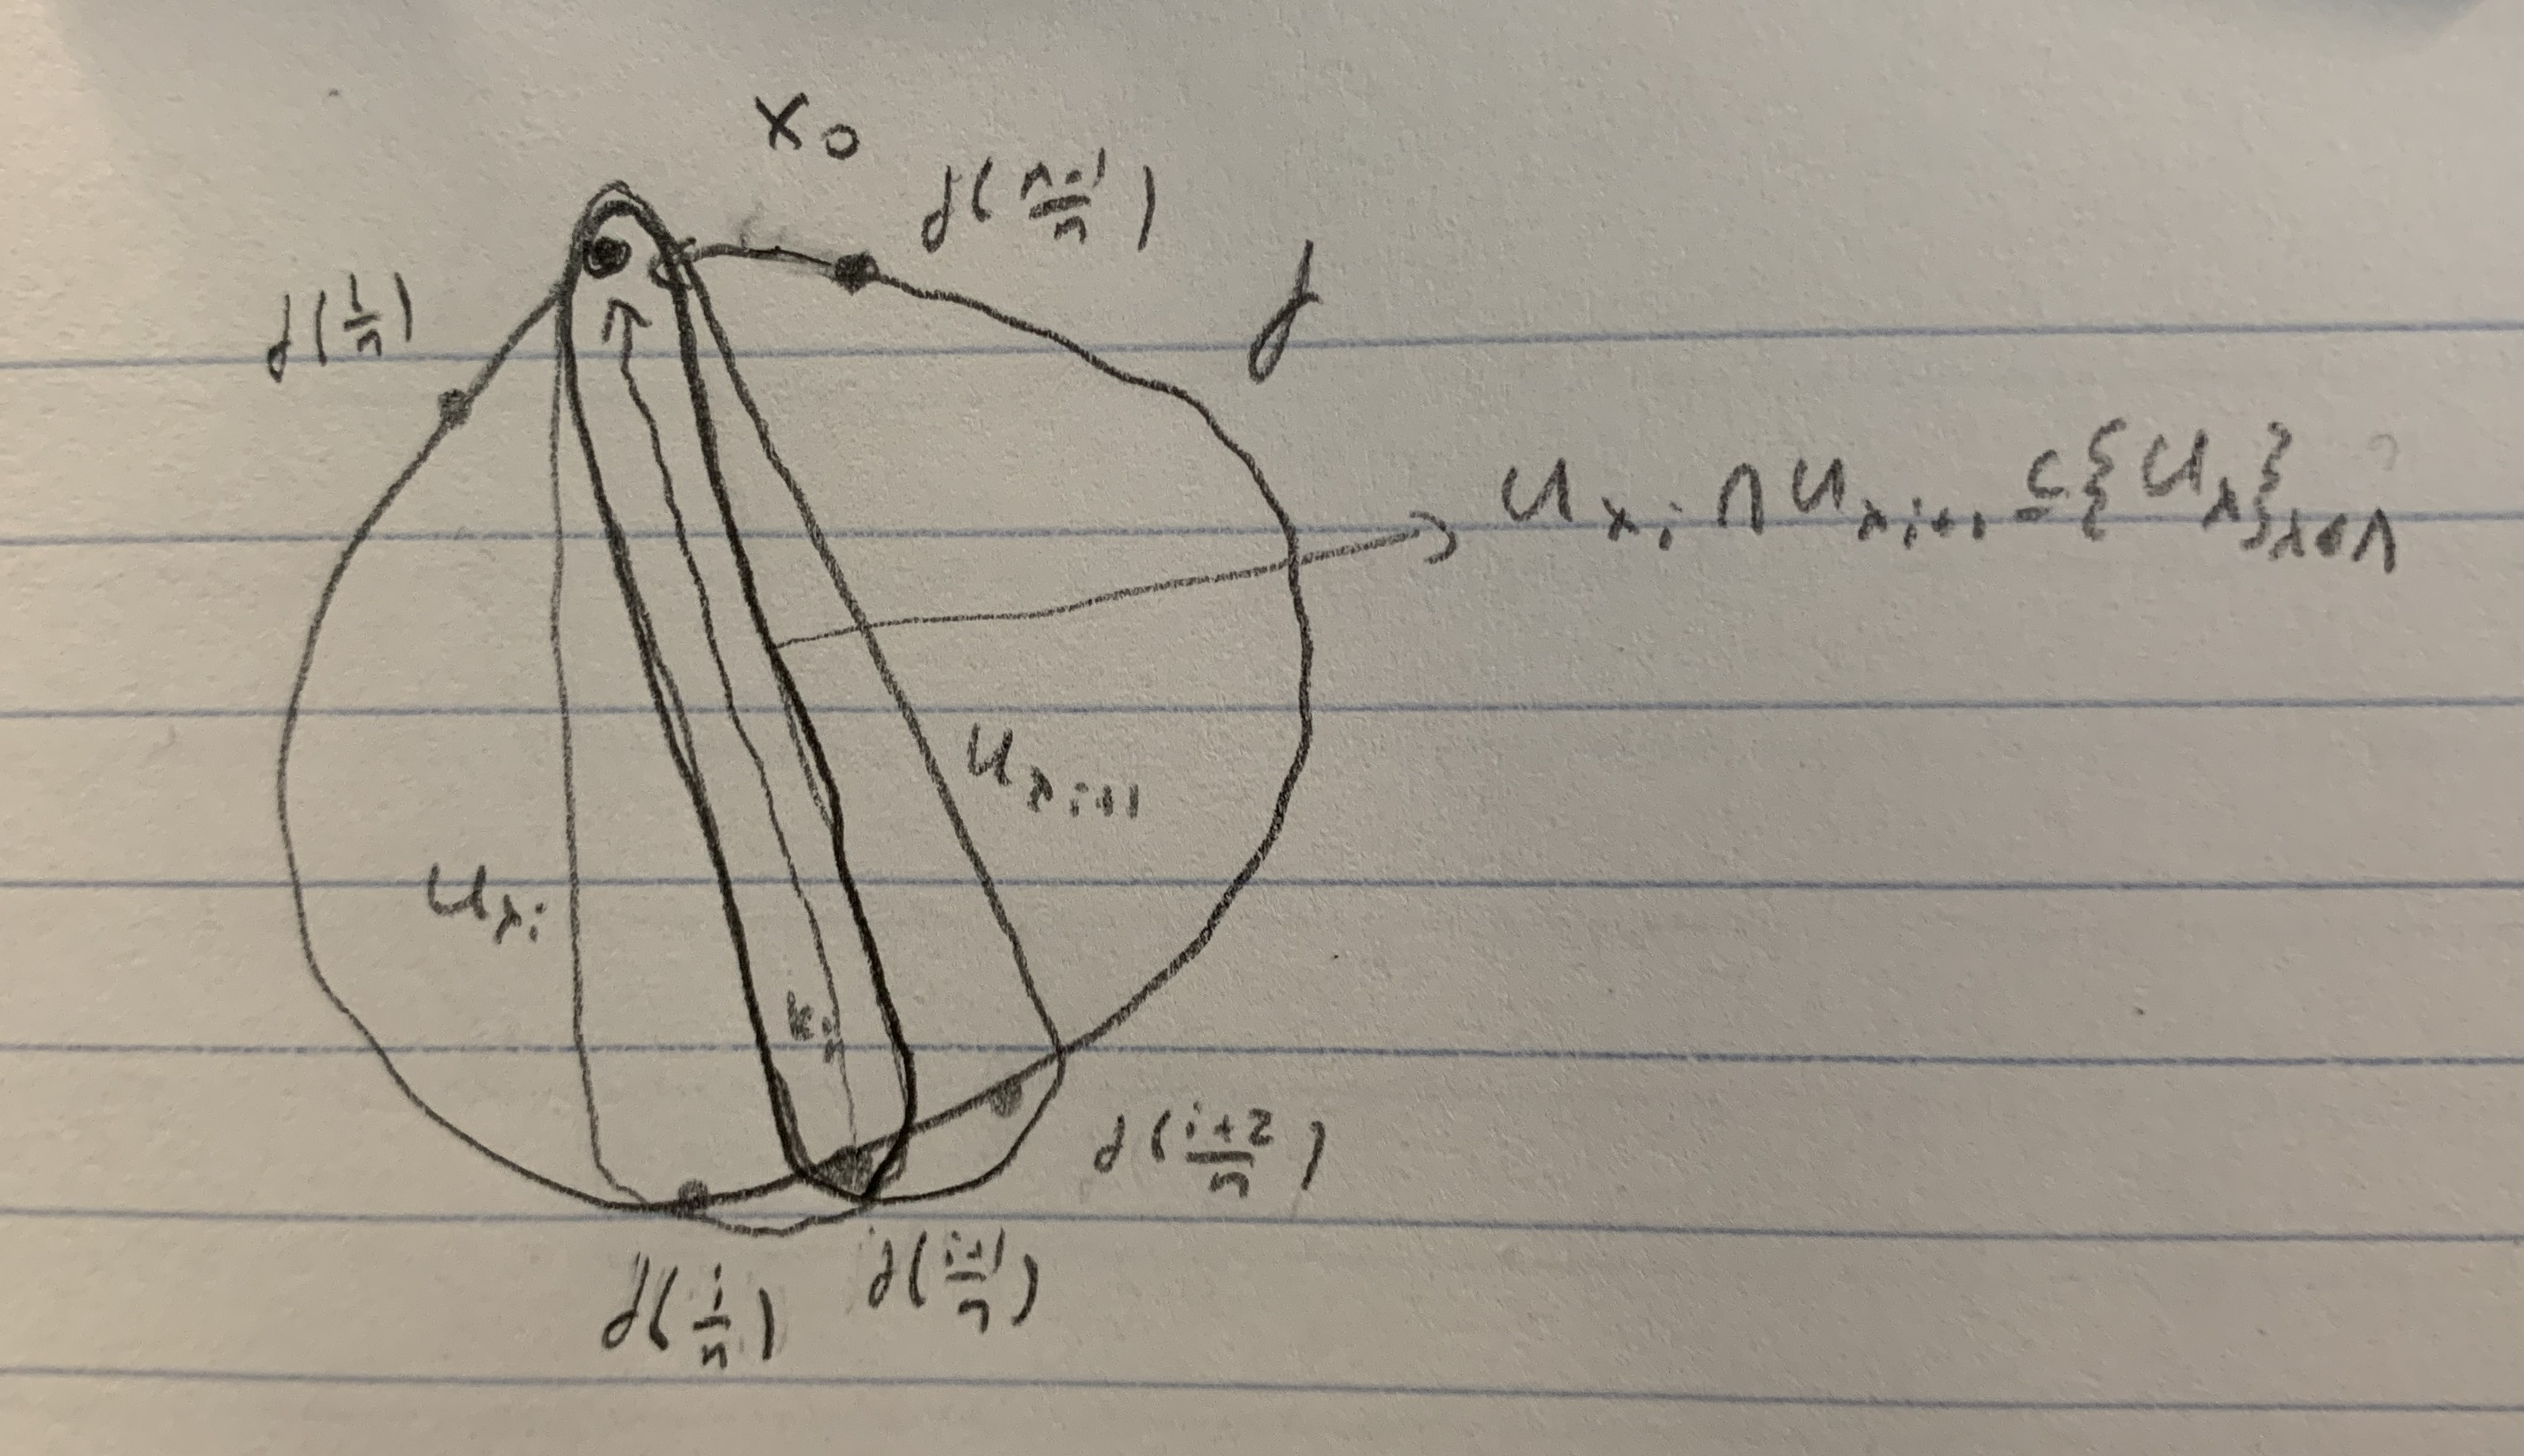
\includegraphics[width=0.7\textwidth]{img/proof-pt1.JPG}<8->
        \end{center}
        \begin{itemize}
          \item<9-> We add the $k_i$ to put each small piece starts and ends at $x_0$,
            and so is in a fundemental group:
              \[f \sim f_1k_1\cdot k_1^{-1}f_2k_2 \cdot k_2^{-1}f_3k_3 \cdot ... \cdot k_{n-1}^{-1}f_n\]
              \[a = [f]_{\pi_1(X)} = [f_1k_1]_{\pi_1(X)} [k_1^{-1}f_2k_2]_{\pi_1(X)}
                 ... [k_{n-1}^{-1}f_n]_{\pi_1(X)}\]
            Now, $k_{i-1}f_ik_i \subseteq U_{\lambda_i}$, since $k_i \subseteq
            U_{\lambda_i}, U_{\lambda_{i+1}}$. Since $\psi_{\lambda_i}$ is the
            homomorphism induced by an inclusion map,
              \[ a = \psi_{\lambda_1}([f_1k_1]_{\pi_1(U_{\lambda_1})}) ...
                \psi_{\lambda_n}( [k_{n-1}f_n]_{\pi_1(U_{\lambda_n})})\]

        \end{itemize}
      \end{column}
    \end{columns}
  \end{frame}
  \begin{frame}
    \frametitle{Seifert -- Van Kampen Theorem Proof -- Part 2}
    \begin{columns}
      \begin{column}[T]{0.5\textwidth}
        \begin{itemize}
          \item<1-> We'd like to show that
              \[\psi_{\lambda_1}(\alpha_1) ... \psi_{\lambda_n}
            (\alpha_n) = \psi_{\mu_1}(\beta_1) ... \psi_{\mu_m}(\beta_m)\]
            Implies
             \[p_{\lambda_1}(\alpha_1) ... p_{\lambda_n}(\alpha_n) =
              p_{\mu_1}(\beta_1) ... p_{\mu_1}(\beta_1) \]

            Since paths are invertible, and everything involved is a homomorphism,
            we can put everything on one side:

            \[\psi_{\lambda_1}(\alpha_1) ... \psi_{\lambda_n}(\alpha_n)
              \psi_{\mu_m}(\beta_m^{-1}) ... \psi_{\mu_1}(\beta_1^{-1}) = 1\]

            Implies
              \[p_{\lambda_1}(\alpha_1) ... p_{\lambda_n}(\alpha_n)
              p_{\mu_m}(\beta_m^{-1}) ... p_{\mu_1}(\beta_1^{-1}) = 1\]

          \item<2-> So, it'll suffice to show,
            $\psi_{\lambda_1}(\alpha_1) ... \psi_{\lambda_n}(\alpha_n) = 1$ implies
            $p_{\lambda_1}(\alpha_1) ... p_{\lambda_n}(\alpha_n) = 1$

          \item<3-> Let $f_i$ represent $\psi_{\lambda_i}(\alpha_i)$ so
            $\psi_{\lambda_i}(\alpha_i) = [f_i]_{\pi_1(X)}$.
          \item<4-> If $\psi_{\lambda_1}(\alpha_1) ... \psi_{\lambda_n}(\alpha_n) = 1$,
            there's a continuous function $F : [0,1]x[0,1] \rightarrow X$ with
            $F(1,t) = F(s,0) = F(s,1) = x_0$,
            \[F(0,t) = \begin{cases} f_1 & [0,\frac{1}{n}) \\ f_2 & [\frac{1}{n}, \frac{2}{n}) \\ ... \end{cases}\]

        \end{itemize}
      \end{column}
      \begin{column}[T]{0.5\textwidth}
        \begin{itemize}
          \item<5-> Using the Lebesgue number, split up $[0,1]x[0,1]$ into rectangles
            so each fits in a single $U_\lambda$, making sure that each $\frac{i}{n}$ is at a boundary:
            \begin{center}
              \includegraphics[width=0.4\textwidth]{img/proof-pt2-intro.JPG}<6->
            \end{center}
          \item<7-> For each intersection, add a line $k_{ij}$ going from the intersection to $x_0$, contained in the $U_\lambda$'s of all four surrounding rectangles.
          \item<8-> In each line below, add $k_{ij}$'s as necessary to put them in the fundemental group:

            For each rectangle, since it's contained in $U_\lambda$,
            \begin{center}
              \includegraphics[width=0.7\textwidth]{img/proof-pt2-1.JPG}<9->
            \end{center}

          \end{itemize}
      \end{column}
    \end{columns}
  \end{frame}
  \begin{frame}
    \begin{columns}
      \begin{column}[T]{0.5\textwidth}
        \begin{itemize}
          \item<1-> Now, remember that
            \[\begin{tikzcd}[ampersand replacement=\&]
              \pi_1(U_\lambda) \ar[rd, "p_\lambda"]
              \ar[r,"\phi_{\lambda\mu}"] \& \pi_1(U_\mu) \ar[d, "p_\mu"]\\
                  \& H
              \end{tikzcd}\]
            \begin{center}
              \includegraphics[width=0.5\textwidth]{img/proof-pt2-2.JPG}<2->
            \end{center}

          \item<3-> Notice that along the left, top, and right edges, $p$ of the trivial
            loops is $1$, so the whole composition is $1$.

          \item<4-> Now, we can apply the previous two parts a finite number of times to
            move that composition to the bottom without changing its value:


        \end{itemize}
      \end{column}
      \begin{column}[T]{0.5\textwidth}
            \begin{center}
              \includegraphics[width=0.7\textwidth]{img/proof-pt2-final.JPG}<5->
            \end{center}
        \begin{itemize}
          \item<5-> And that concludes the proof of Seifert-Van Kampen theorem: We
            proved that $\sigma$ is well-defined, so it exists, and we know that
            it's unique.
        \end{itemize}
      \end{column}
    \end{columns}
  \end{frame}
  \begin{frame}
    \frametitle{Seifert -- Van Kampen Theorem, corollary}

    \begin{columns}
      \begin{column}[T]{0.5\textwidth}
        \begin{itemize}
          \item<1-> We will prove: If $X = U \cup V$, $\pi(X) = \frac{\pi(U) *
            \pi(V)}{N}$ where $N$ is the smallest subgroup containing $\phi_{U
            \cap V, U}(x)\phi_{U \cap V, V}(x)^{-1}$ for all $x$ in $U \cap V$.
          \item<2-> Elements of the free product $\pi(U) * \pi(V)$ are strings like
            $u_1v_1u_2..v_n$, where each $u_i$ is in $\pi(U)$ and each $v_i$ is
            in $\pi(V)$. If two adjacent elements are in the same group, you can
            apply that group's operation:
            \[u_1u_2v_1 = (u_1 \cdot_{\pi_U}u_2)v_3\]
            
            In terms of generators and relations, if $\pi(U) = \langle u_1, u_2,
            ...: r_1, r_2, ...\rangle $, $\pi(V) = \langle v_1, v_2, ...: r'_1,
            r'_2, ...\rangle $, and $\pi(U \cap V) = \langle w_1, w_2, ...:
            r''_1, r''_2, ...\rangle $, then
          \[\pi(U)*\pi(V) = \langle u_1, u_2, ..., v_1, v_2, ... : r_1, r_2,
            ..., r'_1, r'_2, ...\rangle \]
          \[\frac{\pi(U) * \pi(V)}{N} = \langle u_1, ..., v_1, ... : r_1, ...,
            r'_1, ..., i_U(w_1)i_V(w_1)^{-1}, ...\rangle \]

          \item<3-> Proof: We can define a function $F : \pi(U) * \pi(V) \rightarrow \pi(X)$, by
            \[F(u_1v_1u_2...v_n) = \psi_U(u_1)\psi_V(v_1)\psi_U(u_2) ... \psi_V(v_n)\]
            If $i_U(x)i_V(x)^{-1} \in N$,
            \[F(i_U(x)i_V(x)^{-1}) = \psi_U(i_U(x))\psi_V(i_V(x))^{-1} = 1\]
          \end{itemize}
        \end{column}
        \begin{column}[T]{0.5\textwidth}
          \begin{itemize}

            \item<4-> So, $N$ is in the kernel of $F$ and the function $F$ is well
              defined $\frac{\pi(U)*\pi(V)}{N} \rightarrow \pi(X)$.
              By the proof of Seifert - Van Kampen's theorem, part 1, we know
              that elements $\psi_U(u_1)\psi_V(v_1)\psi_U(u_2) ... \psi_V(v_n)$
              generate $\pi(X)$, so $F$ is surjective onto $\pi(X)$.
              We also have:
              \[i_1: \pi(U) \rightarrow \frac{\pi(U)*\pi(V)}{N}, i_1(u) = u\]
              \[i_2: \pi(V) \rightarrow \frac{\pi(U)*\pi(V)}{N}, i_1(v) = v\]
              \[i_3: \pi(U \cap V) \rightarrow \frac{\pi(U)*\pi(V)}{N}, i_1(x)
              = i_U(x) = i_V(x)\]
            where the last two elements are equal in the quotient group since
              $i_U(x)i_V(x)^{-1} \in N$.

          \item<5-> Then, we can apply Seifert - Van Kampen's theorem and get
            $\sigma :
              \pi(X) \rightarrow \frac{\pi(U)*\pi(V)}{N}$.
            The following commutes:
            \[\begin{tikzcd}[ampersand replacement=\&]
                \pi_1(U) \ar[rd, "i_1"] \ar[r, "i_U"] \&
                \pi_1(X) \ar[d, "\sigma"] \\ \& H \end{tikzcd}\]
          \end{itemize}
        \end{column}
    \end{columns}
  \end{frame}
  \begin{frame}
    \begin{columns}
      \begin{column}[T]{0.5\textwidth}
        \begin{itemize}
          \item<1-> The following commutes:
            \[\begin{tikzcd}[ampersand replacement=\&]
                \pi_1(U) \ar[rd, "i_1"] \ar[r, "i_U"] \&
                \pi_1(X) \ar[d, "\sigma"] \\ \& H \end{tikzcd}\]
          \item<2->
            Elements of $\pi(U)$ and $\pi(V)$ generate $\pi(U)*\pi(V)$,
            which generates $\frac{\pi(U)*\pi(V)}{N}$.
          \item<3->
            If $u \in \pi(U)$, 
            \[(\sigma \cdot F)(u) = \sigma(i_U(u)) = i_1(u) = u\]
            Similarly, if $v \in \pi(U)$,
            \[(\sigma \cdot F)(v) = \sigma(i_V(u)) = i_2(v) = v\]
          \item<4-> Then, this means $\sigma \cdot F$ is the identity function.
          \item<5-> Then, $F$ is injective.
          \item<6-> We already knew $F$ was surjective, so $F$ is an isomorphism and
            the groups $\pi(X)$ and $\frac{\pi(U)*\pi(V)}{N}$ are isomorphic.
        \end{itemize}
      \end{column}
      \begin{column}[T]{0.5\textwidth}
        \begin{itemize}
          \item<7-> To conclude,
          \[\pi(X) = \langle u_1, ..., v_1, ... : r_1, ...,
            r'_1, ..., i_U(w_1)i_V(w_1)^{-1}, ...\rangle \]
        \[= \langle u_1, ..., v_1, ... : r_1, ...,
            r'_1, ..., i_U(w_1)=i_V(w_1), ...\rangle \]
          where
            \[\pi(U) = \langle u_1, u_2, ...: r_1, r_2, ...\rangle \]
            \[\pi(V) = \langle v_1, v_2, ...: r'_1, r'_2, ...\rangle \]
            \[\pi(U \cap V) = \langle w_1, w_2, ... :r''_1, r''_2, ...\rangle\]
        \end{itemize}
      \end{column}
    \end{columns}
  \end{frame}
            
  \begin{frame}
    \frametitle{Calculating the group of the trefoil knot}
    \begin{columns}
      \begin{column}[T]{0.5\textwidth}
        \begin{itemize}
          \item<1-> We'll consider the trefoil knot we saw in the introduction.
          \item<2-> We can draw it on a torus:
          \item<3-> Then, split the space $R^3 - K$ into three sections:
          
            $A$: inside the torus, including the boundary (but not $K$)

            $B$: outside the torus, including the boundary (but not $K$)

            $A \cap B$: the boundary of the torus, not including $K$.

          \item<4-> The fundemental group of $A$ is essentially the same as the fundemental
          group of $S^1$, which is $\langle u\rangle $, where $u$ is a loop going aroung the hole

          \item<5-> The fundemental group of $B$ is essentially the same as the fundemental group
            of $R^3 - S^1$, which we saw is $\langle v\rangle $ where $v$ is the loop in the picture:

          \item<6-> $A \cap B$ is essentially just a strip in $R^3$, so its
            fundemental group is going around once in the strip, $\langle w\rangle $.

          \item<7-> $w$ goes around the torus two times, so $i_U(w) = u^2$. It rotates three times,
            around the outside, so $i_V(w) = v^3$.

          \item<8-> By Seifert -- Van Kampen's theorem, $\pi(R^3 - K) = \langle u,v,u^2 = v^3\rangle $
        \end{itemize}
      \end{column}
      \begin{column}[T]{0.5\textwidth}
        \begin{center}
        \includegraphics[width=0.9\textwidth]{img/trefoil-on-torus.JPG}<2->
        \end{center}
        \begin{center}
        \includegraphics[width=0.7\textwidth]{img/AnB.JPG}<3->
        \end{center}
      \end{column}
    \end{columns}
  \end{frame}
  \begin{frame}
    \frametitle{Wirtinger Presentation}
    \begin{columns}
      \begin{column}[T]{0.5\textwidth}
        \begin{itemize}
          \item<1-> Take any 'drawing' of a knot as curves and put it in
            $\mathbb{R}^3$ as shown. Draw lines $a_i$ going across every section
            of the knot.
          \item<2-> At every intersection, there are one of two intersections $r_i$.
          \item<3-> Divide up $\mathbb{R}^3$ as follows:
          \item<4-> $A = \{(x,y,z): z >= -1\}$. In $A$, each line segments forms a
            handle, and the fundemental group of $A$ is going through any number
            of them in any order, so $\langle a_1, ... a_n\rangle $.
          \item<5-> $B_i$: rectangular box under every intersection, with its top at
            $z = -1$. Any path in the rectangular box is trivial, so its fundemental group is $1$.
          \item<6-> $C$: Anything below $A$ and all the $B$'s. Its fundemental group is $1$ as well.

            We'll take $A$ and add the $B_i$'s one by one. $A \cap B_1$ is a
            rectangle with a line segment in the middle cut out. So, its
            fundemental group is generated by going around that line segment
            once, which, included in $A$ is exactly $r_i$. So, the fundemental
            group is $\langle a_1, ... a_n : r_1\rangle $.

            Adding the other $B_i$'s one by one, the fundemental group becomes
            \[\langle a_1, a_2, ... a_n : r_1, r_2, ... r_n\rangle \]
            The intersection of $A \cup B_1 ... \cup B_n$ and $C$ also has a
            trivial fundemental group. So the fundemental group of the union of
            all the parts, $\mathbb{R}^3- K$ is:
            \[\pi(\mathbb{R}^3-K) = \langle a_1, a_2, ... a_n : r_1, r_2, ... r_n\rangle \]

        \end{itemize}
      \end{column}
      \begin{column}[T]{0.5\textwidth}
        \begin{center}
        \includegraphics[width=0.9\textwidth]{img/wirtinger-full.JPG}<1->
        \end{center}
      \end{column}
    \end{columns}
  \end{frame}
  \begin{frame}
    \frametitle{Do we get the same group with the Wirtinger Presentation?}
    \begin{columns}
      \begin{column}[T]{0.5\textwidth}
        \begin{itemize}
          \item<1-> For the trefoil, we get three line segments and three relations
            as shown.
            \[\pi(\mathbb{R}^3-K) = \langle a_1, a_2, a_3: a_1a_3 = a_3a_2, a_2a_1 = a_3a_2, a_2a_1 = a_1a_3\rangle \]
          \item<2->
            Clearly, the first two relations imply the third, so this group is equivalent to
            \[\langle a_1, a_2, a_3: a_1a_3 = a_3a_2, a_2a_1 = a_1a_3\rangle \]
          \item<3->We can solve the first relation for $a_1$ to get $a_1 =
            a_3a_2a_3^{-1}$. So, any string of $a_1$,$a_2$, $a_3$ is also
            generated by $a_2$ and $a_3$ with $a_1$ as this expression. So, we
            get:
            \[\langle a_2, a_3: a_2(a_3a_2a_3^{-1}) = (a_3a_2a_3^{-1})a_3 = a_3a_2\rangle \]
            \[\langle u, v: uvu = vuv\rangle \]
            \[uvu*uvu = vu*vu*vu\]
          \item<5-> Let $w = uvu$, $z = vu$. Then,
            \[u = wz^{-1}, v = zu^{-1} = z(wz^{-1})^{-1} = z^2w^{-1}\]
            So, we can express any string of $u$'s and $v$'s as a string of
            $w$'s and $z$'s, so the group is also generated by $w$ and $z$. Then,
            the relation we have becomes $w^2 = z^3$.
            \[\langle w, z : w^2 = z^3\rangle\]

            And this is the same group we got before.
        \end{itemize}
      \end{column}
      \begin{column}[T]{0.5\textwidth}
        \begin{center}
        \includegraphics[width=0.7\textwidth]{img/wirtinger-torus.JPG}<1->
        \end{center}
      \end{column}
    \end{columns}
  \end{frame}
  \begin{frame}
    \frametitle{Is the group we got actually different than the group of the unknot?}
    \begin{columns}
      \begin{column}[T]{0.5\textwidth}
        \begin{itemize}
          \item<1-> The group of the unknot, $\langle a\rangle $, is commutative -- for any $n, m \in \mathbb{Z}$,
            \[a^na^m = a^{n+m} = a^{m+n} = a^ma^n\]
          \item<2-> We'll argue that the group of the unknot, $B_3 = \langle a,b : a^2 = b^3\rangle $ is not.

          \item<3-> Consider the set $\{1,2,3\}$, and the group of invertible
            functions $\{1,2,3\} \rightarrow \{1,2,3\}$, with the group operation
            being function composition, $S_3$.
          \item<4-> Define $f$ and $g$ as follows:
            \[f(1) = 2, f(2) = 1, f(3) = 3\]
            \[g(1) = 2, g(2) = 3, g(3) = 1\]

            Then,
            \[f^2(1) = 1, f^2(2) = 2, f^2(3) = 3\]
            \[g^2(1) = 3, g^2(2) = 1, g^2(3) = 2\]
            \[g^3(1) = 1, g^3(2) = 2, g^3(3) = 3\]

          \item<5-> So, both are invertible, and so in $S_3$, and in the group,
            $f^2 = g^3 = 1$. Then, since any string of $f$'s and $g$'s is still
            in $S_3$, and $f^2 = g^3$, we can define a homomorphism $\sigma : B_3 \rightarrow S_3$:
            \[\sigma(a) = f, \sigma(b) = g\]
            And this is a well-defined function -- if two different strings are
            the same element in $B_3$, the $\sigma$ of both strings are
            equivalent in $S_3$.
        \end{itemize}
      \end{column}
      \begin{column}[T]{0.5\textwidth}
        \begin{itemize}
          \item<6->
            But,
            \[(fg)(1) = 1, (fg)(2) = 3, (fg)(3) = 2\]
            \[(gf)(1) = 3, (gf)(2) = 3, (gf)(3) = 1\]
          \item<7->  So,
            \[fg \neq gf\]
            \[\sigma(ab) \neq \sigma (ba)\]
            \[ab \neq ba\]
          \item<8->  Since there are elements $a$, $b$ of $B_3$ such that $ab \neq ba$,
            $B_3$ is not commutative, and can't equal $\langle a\rangle $.
          \item<9-> Therefore, the trefoil is a different knot than the unknot.
        \end{itemize}
      \end{column}
    \end{columns}
  \end{frame}
  \begin{frame}
    \frametitle{Sources}
      \begin{itemize}
        \item Gallagher, K. (n.d.). The fundamental group and Seifert-van Kampen’s
          theorem. Retrieved March 6, 2022, from \url{https://www.math.uchicago.edu/~may/REU2016/REUPapers/Gallagher.pdf}
        \item Massey, W. S. (1991). A basic course in algebraic topology. Springer. 
        \item Rolfsen, D. (2003). Knots and links. AMS Chelsea Publ. 
      \end{itemize}

      You can find the source code for this presentation at:

      \url{https://github.com/yahya-tamur/seifert-van-kampen-presentation}
  \end{frame}


\end{document}
